\documentclass[12pt,a4paper]{article}
\usepackage[utf8]{inputenc}
\usepackage[shortlabels]{enumitem}
\usepackage{fontawesome}
%Set page layout parameters
\usepackage[
top=4cm,
bottom=2cm,
left=2cm,
right=2cm,
headheight=2cm,
footskip=1cm,
marginparwidth=2cm]{geometry}
\usepackage{amsmath}
\usepackage{cancel}
\usepackage{hyperref}
\usepackage[dvipsnames]{xcolor}
\usepackage{multicol}
% To use color boxes
\usepackage{tcolorbox}
\usepackage{lipsum}
\tcbuselibrary{listings,theorems,skins,vignette,raster,breakable,magazine,poster,fitting,hooks}
\newcounter{ejemplo}
%Images path
\graphicspath{{images/}}
\usepackage{float} %provide us with the option H
\usepackage{fancyhdr}
\usepackage{tikz}
\usepackage{tikzpagenodes}
%to redefine figure caption 
\renewcommand{\figurename}{Figura}
%change text font
\usepackage[T1]{fontenc}
\usepackage{tgtermes} % LaTeX will use the TEX Gyre Bonum font family 
\hypersetup{
	colorlinks=true,
	linkcolor=blue,
	filecolor=magenta,      
	urlcolor=cyan,
}

\urlstyle{same}
\usepackage{vwcol}
\definecolor{subtitle_yellow}{RGB}{252,213,129}
\definecolor{title_yellow}{RGB}{249,175,16}
\definecolor{steel_blue_title}{RGB}{93,138,168}
\definecolor{pewter_blue_subtitle}{RGB}{149,178,198}
\definecolor{ecru_circle}{RGB}{215,190,130}
\definecolor{ecru_circle1}{RGB}{68,148,173}

\newcommand{\myfirststyle}{%
	\begin{tikzpicture}[remember picture, overlay]
		
		%top border
		\fill[fill=steel_blue_title](current page.north west) rectangle ([yshift=-15mm]current page.north east);
		
		\fill[fill=pewter_blue_subtitle]([yshift=-17mm]current page.north west) rectangle ([yshift=-30mm]current page.north east);
		
		%page box
		%\draw[lightgray, fill=Rhodamine, fill opacity=0.05, line width=1mm, rounded corners=3mm] ([xshift=-5mm,yshift=5mm]current page text area.north west) rectangle ([xshift=5mm,yshift=-5mm]current page text area.south east);
		
		%bottom box
		\fill[fill=pewter_blue_subtitle](current page.south west) rectangle ([yshift=10mm]current page.south east);
		
		%page circle
		\draw[white,fill=ecru_circle1,line width=2mm] ([xshift=-5mm,yshift=25mm]current page text area.north east) circle (1); 
		
		
		%page number text        
		%\node[anchor=center] at ([xshift=-5mm,yshift=25mm]current page text area.north east) {\Huge\bfseries\sffamily\color{white}{\thepage}};
		
		%title text
		\node[anchor=west] at ([yshift=32mm]current page text area.north west) {\Huge\bfseries\sffamily\color{white}{Programar ATTiny85 con Arduino Uno}};
		
		%subtitle text
		\node[anchor=west] at ([xshift=10mm,yshift=16mm]current page text area.north west) {\Large\bfseries\sffamily\color{white}{}};
		
		%footer text
		\node[anchor=center] at ([yshift=-15mm]current page text area.south) {\large\bfseries\sffamily\color{white}{Created by: Rodrigo Castillejos}};
		
	\end{tikzpicture}
}


%create page style
\fancypagestyle{MyFirstStyle}{%
	\fancyhf{}
	\fancyhead[C]{\myfirststyle}
	\renewcommand{\headrulewidth}{0pt}
}%

\pagestyle{MyFirstStyle}

\colorlet{colexam}{red!75!black}
\newtcolorbox[use counter=ejemplo]{myexample}{%
	empty,title={Ejemplo \thetcbcounter},attach boxed title to top left,
	boxed title style={empty,size=minimal,toprule=2pt,top=4pt,
		overlay={\draw[colexam,line width=2pt]
			([yshift=-1pt]frame.north west)--([yshift=-1pt]frame.north east);}},
	coltitle=colexam,fonttitle=\Large\bfseries,
	before=\par\medskip\noindent,parbox=false,boxsep=0pt,left=0pt,right=3mm,top=4pt,
	breakable,pad at break*=0mm,vfill before first,
	overlay unbroken={\draw[colexam,line width=1pt]
		([yshift=-1pt]title.north east)--([xshift=-0.5pt,yshift=-1pt]title.north-|frame.east)
		--([xshift=-0.5pt]frame.south east)--(frame.south west); },
	overlay first={\draw[colexam,line width=1pt]
		([yshift=-1pt]title.north east)--([xshift=-0.5pt,yshift=-1pt]title.north-|frame.east)
		--([xshift=-0.5pt]frame.south east); },
	overlay middle={\draw[colexam,line width=1pt] ([xshift=-0.5pt]frame.north east)
		--([xshift=-0.5pt]frame.south east); },
	overlay last={\draw[colexam,line width=1pt] ([xshift=-0.5pt]frame.north east)
		--([xshift=-0.5pt]frame.south east)--(frame.south west);},%
}

\DeclareTotalTCBox{\commandbox}{ s v }
{verbatim,colupper=pink,colback=black!75!white,colframe=black}
{\IfBooleanT{#1}{\textcolor{cyan}{\ttfamily\bfseries SELECT }}%
	\lstinline[language=command.com,keywordstyle=\color{blue!35!white}\bfseries]^#2^}

\DeclareTotalTCBox{\commandboxa}{ s v }
{verbatim,colupper=white,colback=gray!75!white,colframe=gray}
{\IfBooleanT{#1}{\textcolor{cyan}{\ttfamily\bfseries SELECT }}%
	\lstinline[language=command.com,keywordstyle=\color{blue!35!white}\bfseries]^#2^}

\begin{document}
	\newtcbox{\fancybox}[1][red]{on line,arc=0pt,outer arc=0pt,colback=#1!10!white,colframe=#1!50!black,boxsep=0pt,left=1pt,right=1pt,top=2pt,bottom=2pt,boxrule=0pt,bottomrule=1pt,toprule=1pt}
	\newtcbox{\xmybox}[1][red]{on line,arc=7pt,colback=#1!10!white,colframe=#1!50!black,before upper={\rule[-3pt]{0pt}{10pt}},boxrule=1pt,boxsep=0pt,left=6pt,right=6pt,top=2pt,bottom=2pt}
	
	Este tutorial muestra cómo programar el ATTiny85 desde el IDE de Arduino con la ayuda de la tarjeta Arduino Uno.
	
	Por defecto, el IDE de Arduino no soporta la gama de microcontroladores ATTiny, por lo que será necesario agregar dicho soporte, a continuación se muestran los pasos.\\
	
	En nuestro IDE de Arduino, seleccionamos la opción \verb|Archivo > Preferencias|, o bien, podemos, usar la combinación de teclas \commandboxa{Ctrl + coma} (figura \ref*{fig:preferencias})
	\begin{figure}[H]
		\centering
		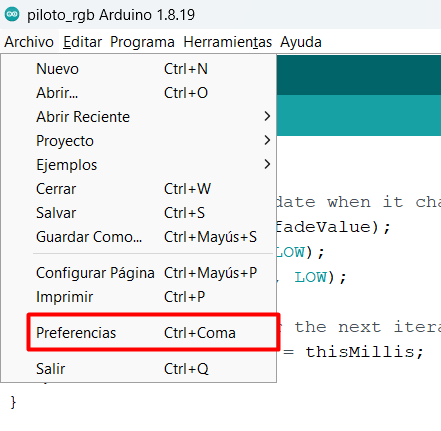
\includegraphics[scale=0.8]{preferencias}
		\caption{}
		\label{fig:preferencias}
	\end{figure}

	En el cuadro de diálogo \verb|Preferencias|, dentro de \textbf{Gestor de URLs Adicionales de Tarjetas} colocamos la siguiente URL (figura \ref{fig:gestor_de_tarjetas}). Damos clic en \commandboxa{Ok} y reiniciamos el IDE de Arduino.
	\begin{figure}[H]
		\centering
		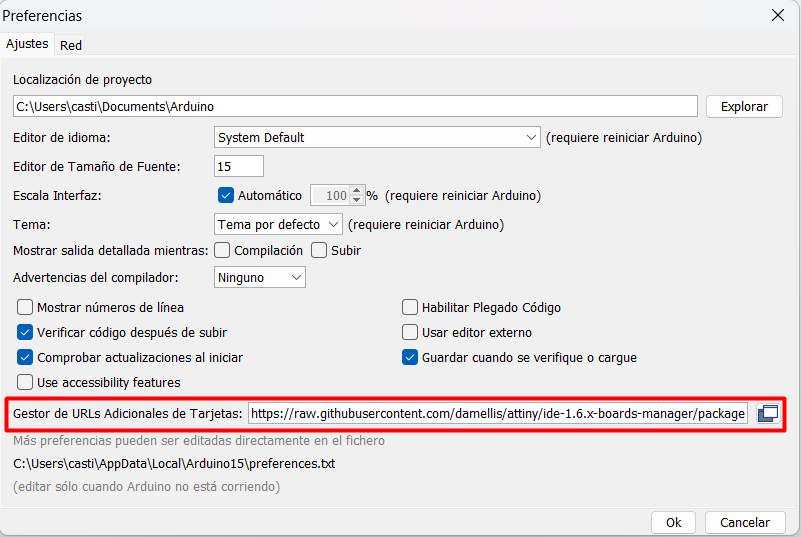
\includegraphics[scale=0.7]{gestor_de_tarjetas}
		\caption{}
		\label{fig:gestor_de_tarjetas}
	\end{figure}
	\begin{tcolorbox}[colback=yellow!10!white,colframe=yellow!50!black,title=URL]
		\url{https://raw.githubusercontent.com/damellis/attiny/ide-1.6.x-boards-manager/package_damellis_attiny_index.json}
	\end{tcolorbox}

	Abrimos nuevamente nuestro IDE de Arduino y en \verb|Herramientas| buscamos la opción denominada \verb|Gestor de tarjetas| (figura \ref{fig:gestor_de_tarjetas_op}).
	\begin{figure}[H]
		\centering
		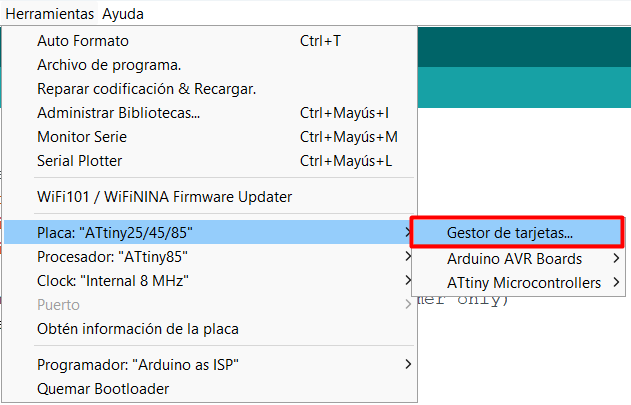
\includegraphics[scale=0.7]{gestor_de_tarjetas_op}
		\caption{}
		\label{fig:gestor_de_tarjetas_op}
	\end{figure}

	Dentro del cuadro de diálogo \verb|Gestor de Tarjetas| escribimos \textbf{ATTiny} e instalamos el paquete.
	\begin{figure}[H]
		\centering
		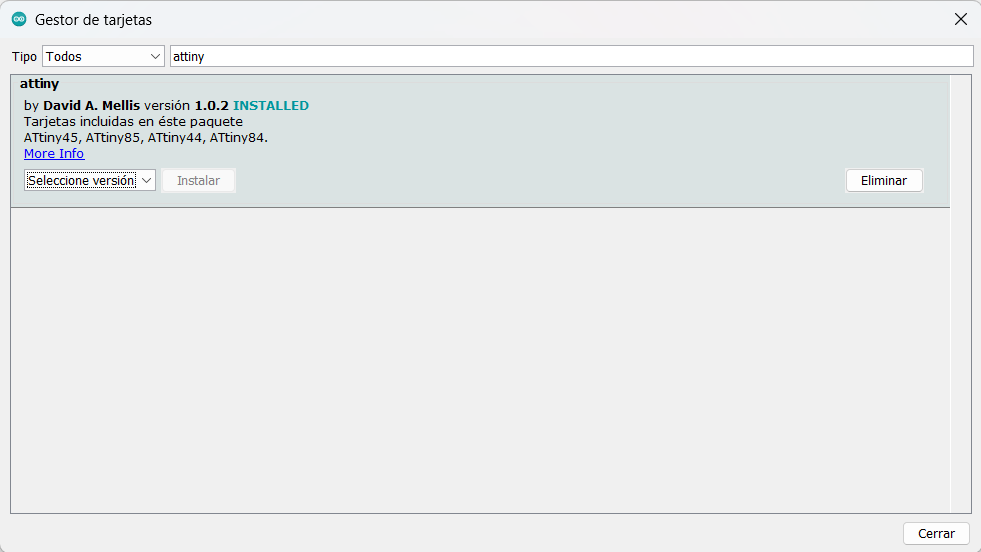
\includegraphics[scale=0.7]{looking_for_attiny}
		\caption{}
		\label{fig:looking_for_attiny}
	\end{figure}

	Ya que nuestra meta es ser capaces de programar el ATTiny desde el IDE de Arduino, el cual requiere quemar el Bootloader al ATTiny85, necesitamos primero preparar el Arduino cargando el programa \textbf{ArduinoISP} a nuestro microcontrolador ATMega328P.
	
	\newpage
	
	En \verb|Archivos|, en el apartado de \verb|Ejemplos|, buscamos el ejemplo \verb|11.ArduinoISP| (figura \ref{fig:ArduinoISP})
	\begin{figure}[H]
		\centering
		\includegraphics[scale=0.7]{ArduinoISP}
		\caption{}
		\label{fig:ArduinoISP}
	\end{figure}

	Conectamos nuestro Arduino UNO, verificamos que sea la tarjeta correcta y el puerto indicado, posteriormente verificamos y cargamos el programa como se muestra en la figura 
	\begin{figure}[H]
		\centering
		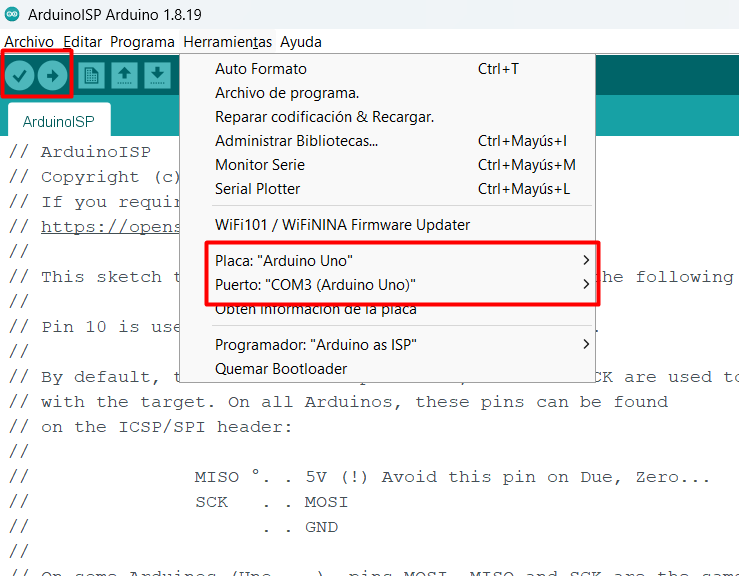
\includegraphics[scale=0.7]{upload_arduinoISP}
		\caption{}
		\label{fig:upload_arduinoISP}
	\end{figure}

	\newpage
	
	Ahora realizamos la conexión que se muestra en la figura 
	\begin{figure}[H]
		\centering
		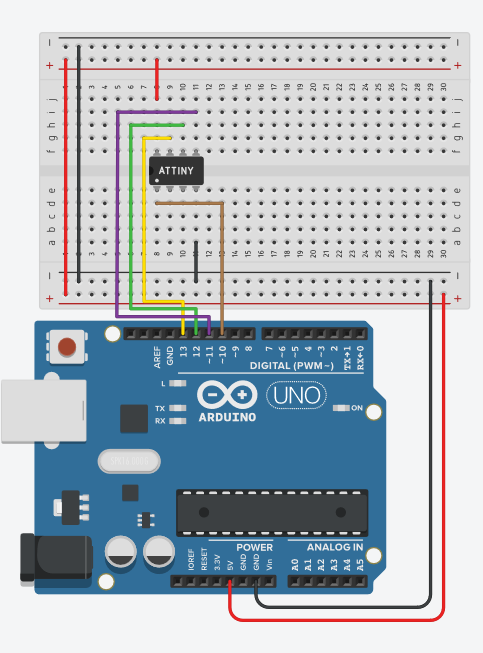
\includegraphics[scale=1]{conexion1}
		\caption{}
		\label{fig:conexion1}
	\end{figure}
\end{document} 

